\section{Transmitter schematics}

The top-level schematic of our transmitter circuit is shown in figure \ref{fig:top_level}. To make the circuit simpler to read, blocks are used for the different parts and the schematics of these blocks are shown separately. The input flipflops are implemented as in figure \ref{fig:flipflop}. Figure \ref{fig:slices} contains the schematics of our output slices. Note that each differential slice (part a of figure \ref{fig:slices}) contains two single-ended slices (part b of figure \ref{fig:slices}). All used gates were implemented on transistor level as well, the schematics for them are shown in figure \ref{fig:gates}.\\


%TODO explain sizing!! and give the values!

\begin{figure}[ht]
  \centering
  {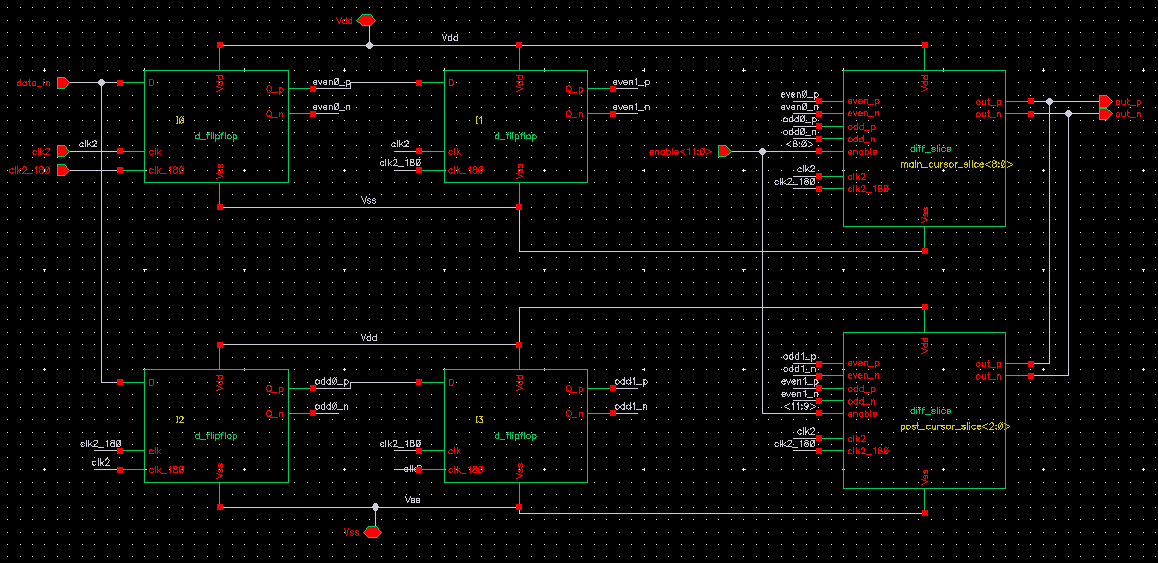
\includegraphics[scale=0.55]{img/transmitter.png}}
  \caption{Transmitter top level circuit}
  \label{fig:top_level}
\end{figure}

\begin{figure}[ht]
  \centering
  \subfigure[Differential slice]
  {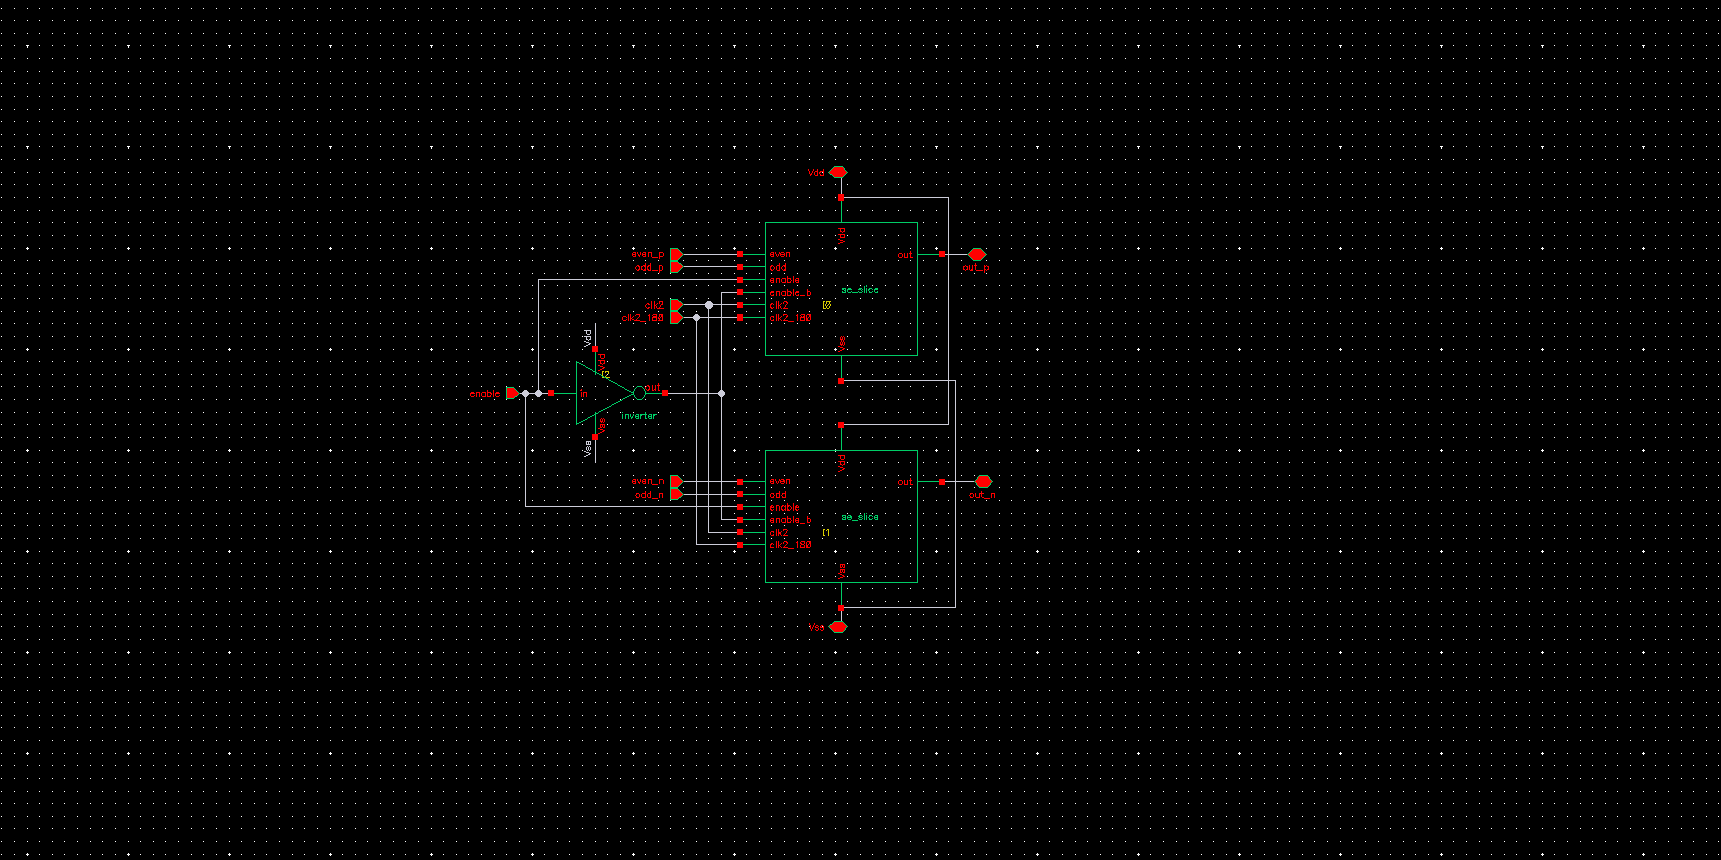
\includegraphics[scale=0.6]{img/diff_slice.png}}
  \subfigure[Single-ended slice]
  {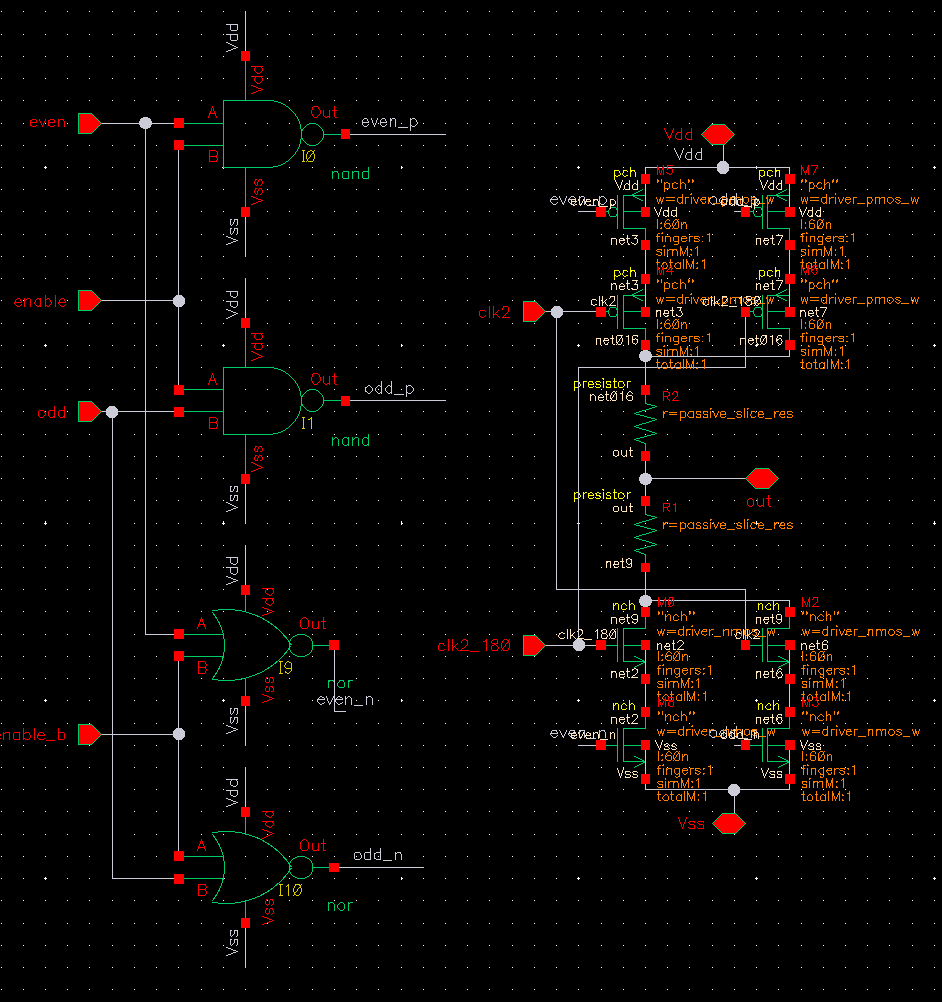
\includegraphics[scale=0.5]{img/se_slice.png}}
  \caption{Slice circuits}
  \label{fig:slices}
\end{figure}

\begin{figure}[ht]
  \centering
  {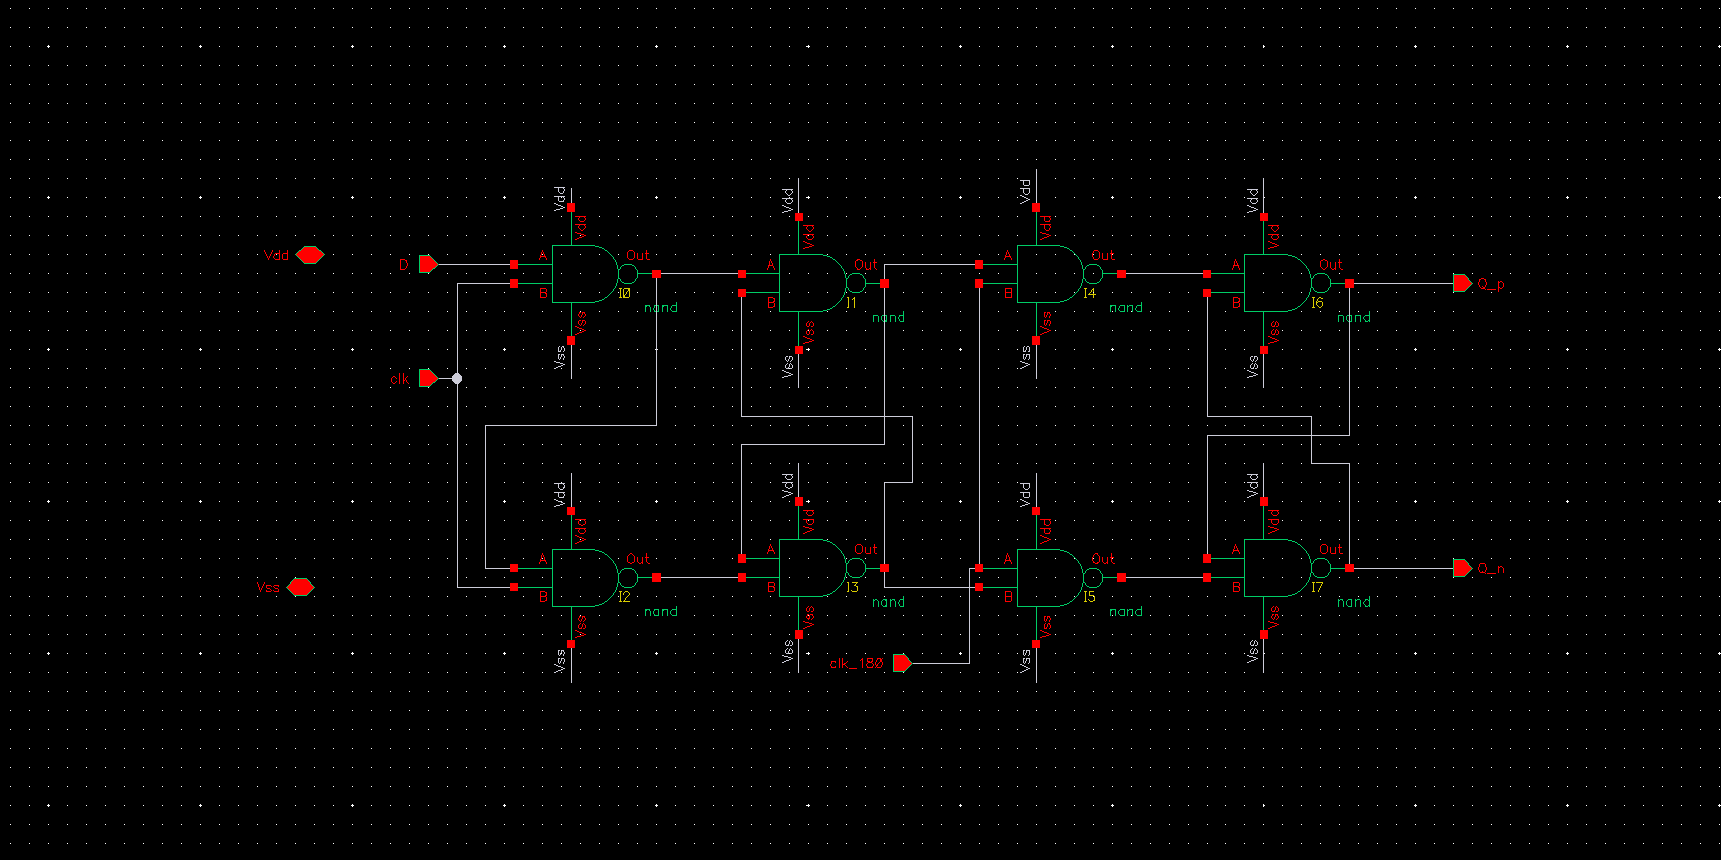
\includegraphics[scale=0.47]{img/flipflop.png}}
  \caption{D-Flipflop}
  \label{fig:flipflop}
\end{figure}

\begin{figure}[ht]
  \centering
  \subfigure[Inverter]
  {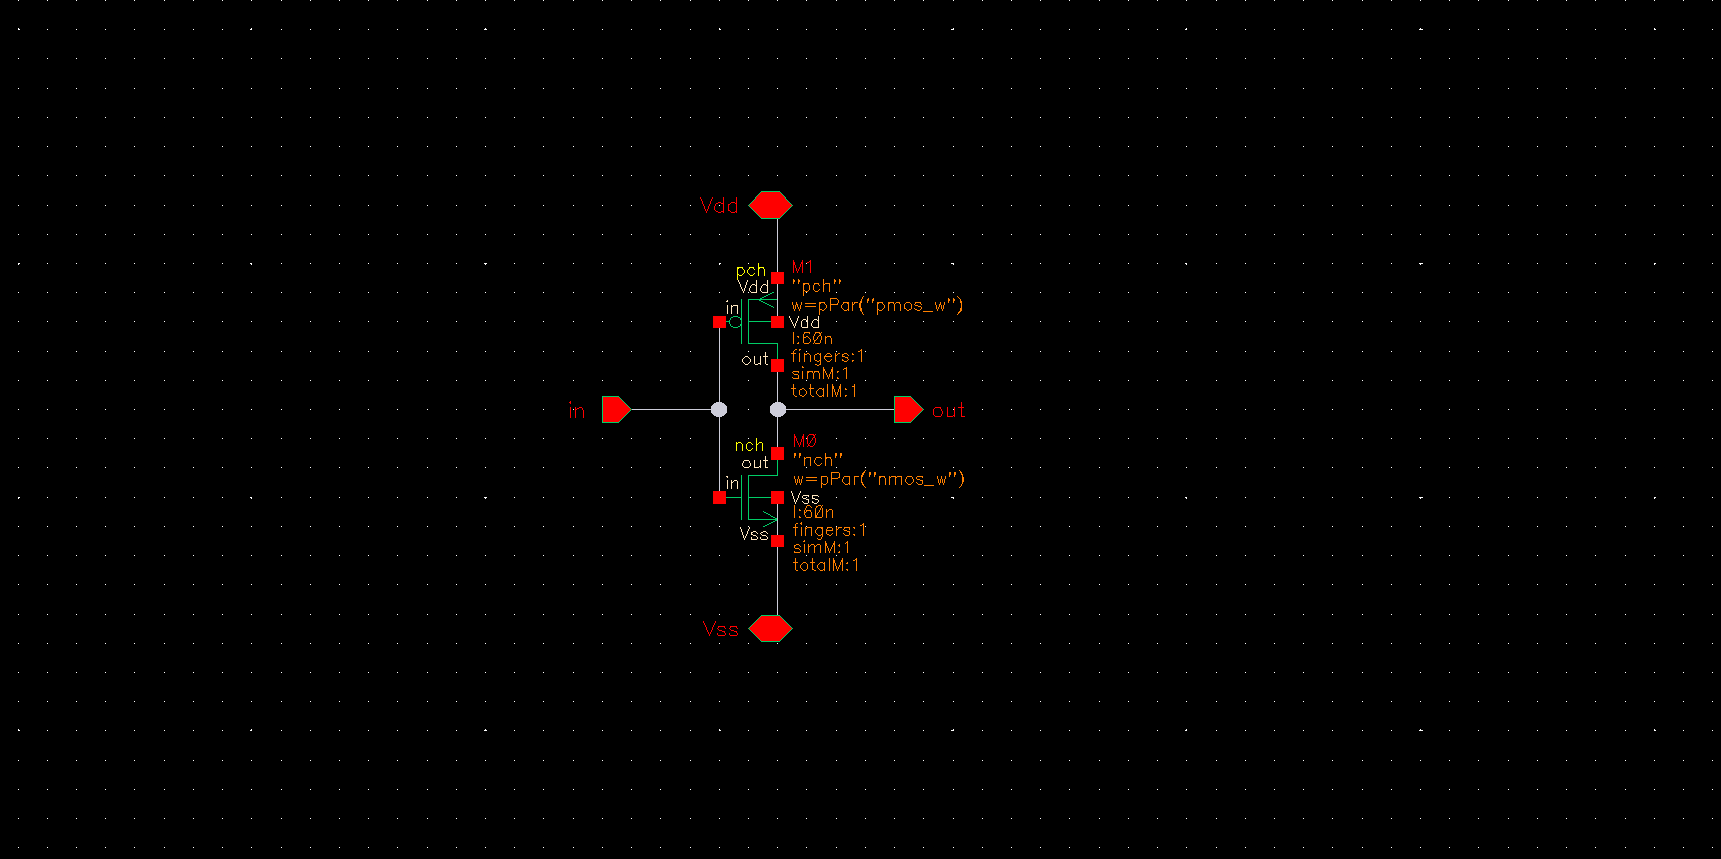
\includegraphics[scale=0.5]{img/inverter.png}}
  \subfigure[NAND gate]
  {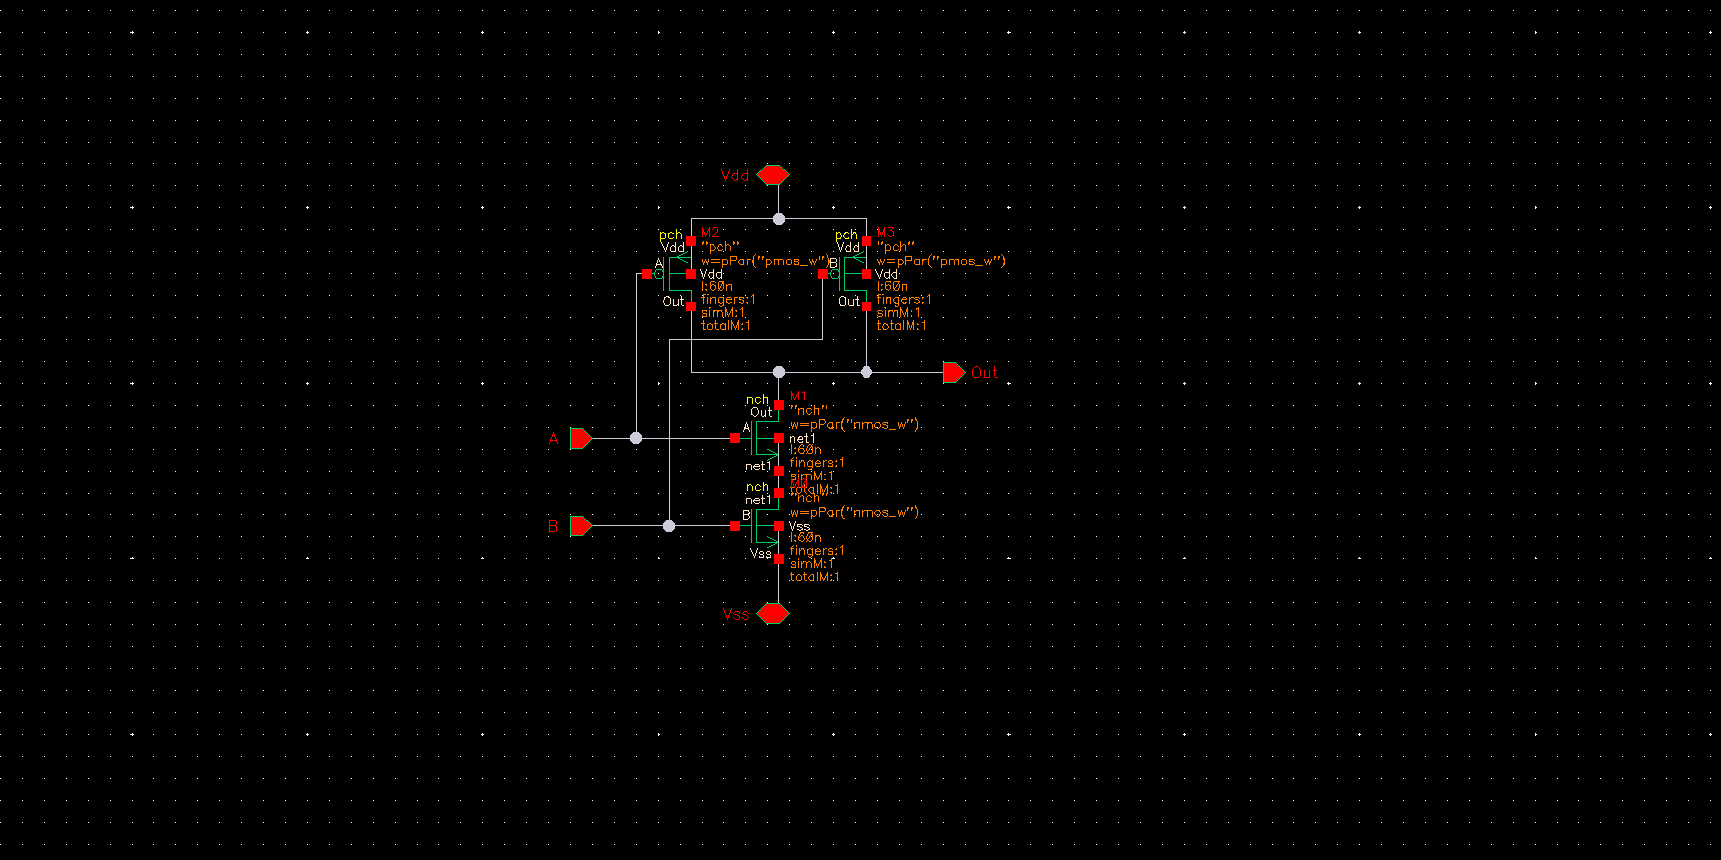
\includegraphics[scale=0.5]{img/nand.png}}
  \subfigure[NOR gate]
  {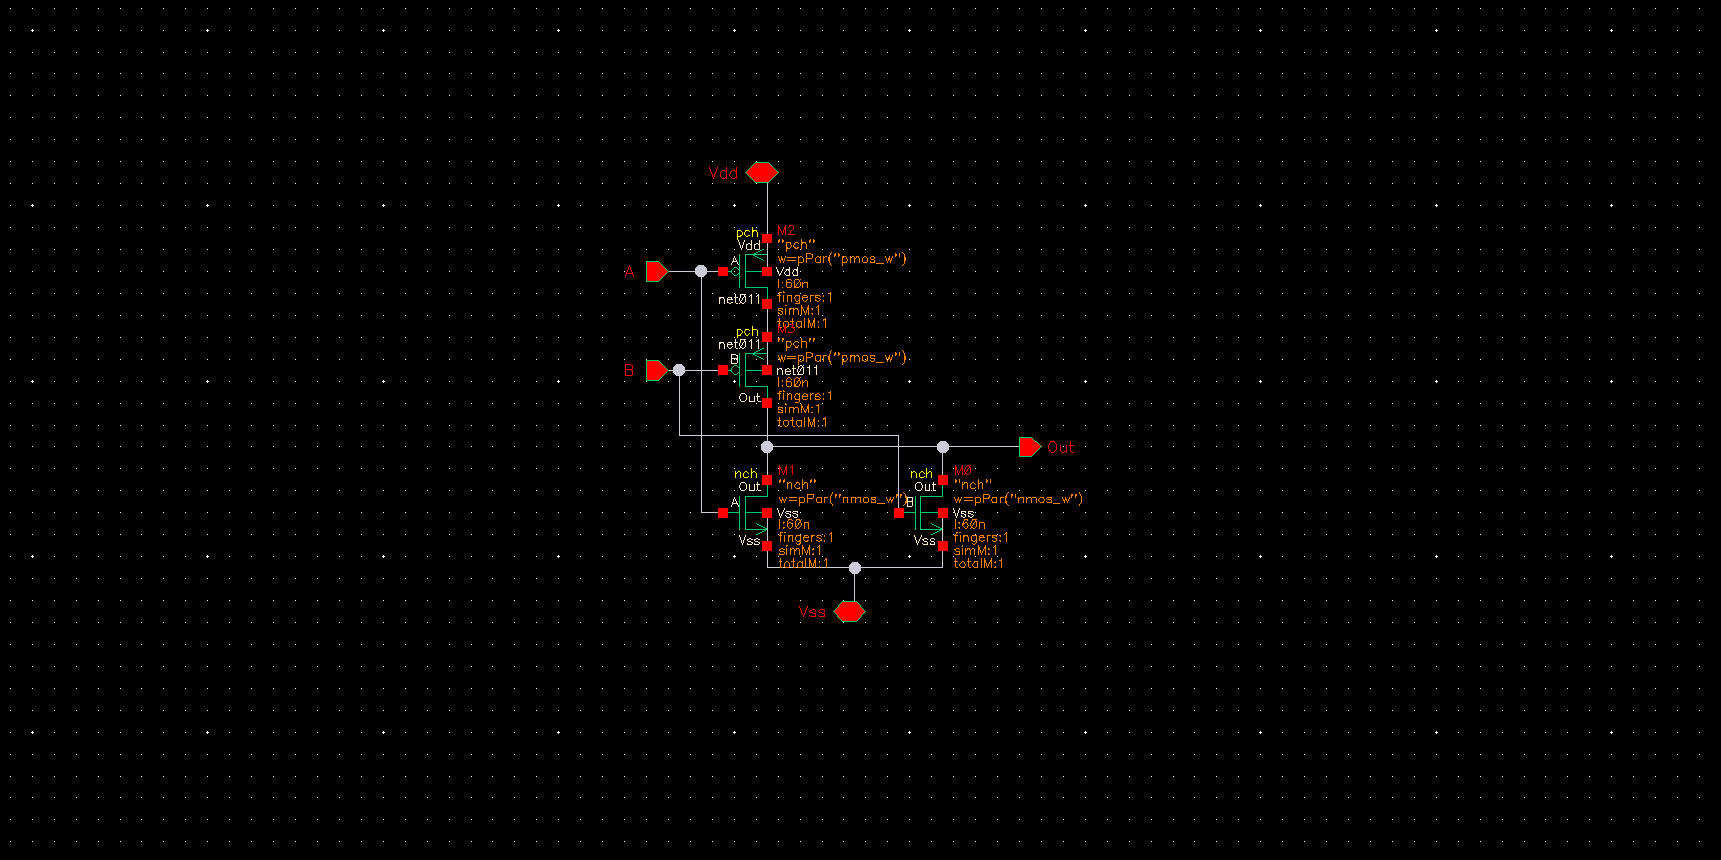
\includegraphics[scale=0.5]{img/nor.png}}
  \caption{Simple gate circuits}
  \label{fig:gates}
\end{figure}